\section{Methods}
Over a five year period, a process was created and refined that eventually became a framework for employing students as software developers for the purpose of developing software for an academic institution. Following best practices in Agile and lean thinking, the framework is constantly being evaluated, redesigned, and optimized each year. Thus, the framework presented in this section represents the current state of the framework, generalized as much as possible, and kept at a high-level. It will certainly change as needs of the team and the institution change. Figure \ref{framework} illustrates the framework. 

\subsection{The Summer Internship}
Starting with the summer term, students are hired into the Student Software Development Team (SSDT). Students apply in the previous spring term through an application process. The students are then hired based on a few key metrics, including grades in key classes, such as the CS1 course; their ability to work well with others (based on their interactions with other students in classes, which follow a team-based \cite{2002PairProgramming}, active learning pedagogy \cite{2012Pogil}; and the perceived value they will attain from participating in the program (i.e., the best computer science students are not always selected, as they may not benefit as much from the program). 

% NEEDS IMAGE!
%Check slack -Kat
\begin{figure}[h]
  \centering
  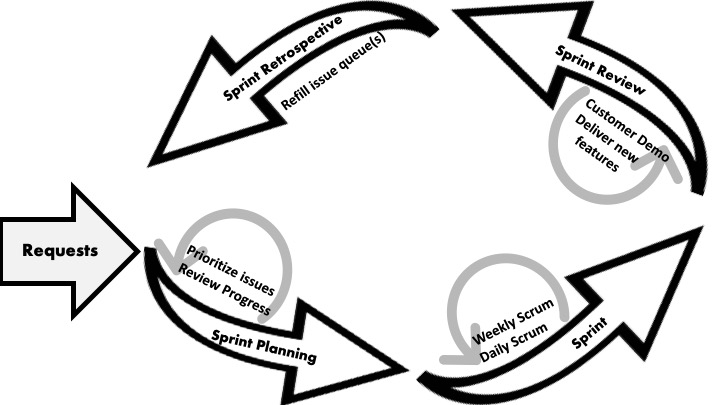
\includegraphics[width=\linewidth]{developmentcycle3.jpg}
  \caption{The Student Software Development Framework}
  \Description{The Student Software Development Framework}
\end{figure}

A typical summer operates much like an internship outside of the academic institution. Students are employed for 40 hours per week for eight to ten weeks, resulting in up to 400 hours of software engineering experience just in the summer. During this time, their expectations mirror an internship in many ways, in that they are expected to show up at work on time, be productive throughout the day, and report back to supervisors of their progress. Each summer consists of six to ten students managed by 2 supervisors (one faculty, one staff). The student typically work in pairs as they design interfaces and develop code. 
Teams  of  students  start  in  the  summer,  working  approximately 400 hours under the supervision of a faculty member, where they are trained on the software engineering principles and apply  them  to  in-progress  projects  or  new  ones.  The  projects  are proposed by the campus community (a.k.a. the customer) and are then selected by the faculty member supervising the team. These projects are often tools requested by the customer to help them complete their daily work, and thus, the software becomes an crucial part of the customer’s job. 

During the summer term, students wok together to take customer needs into consideration as they design new interfaces; they do so through a process called paper prototyping. This consists of many iterations of interfaces on paper rather than writing code first; designs are critiqued and modified until there is a group consensus to move forward. The interface is a sheet of paper with all the elements of the page present. Toward the beginning of this process, the supervising faculty member will act as the "driver", meaning that they "click- through" the interface, while those who designed the prototype will move pieces of the interface to act out its functionality. The first draft typically acts as an eye-opener for the students; the driver finds many flaws and functionalities that their designs are missing. After the first drafts are critiqued, the teams continue to modify and demo their interfaces until the group approves of them. From there, teams make a list of all the pieces of data their interfaces will need. The group participates in a model-building session in which they propose the underlying data structures(s) of the application.%How deep into MVC do we wanna go here..? - Kat
After the model are determined, the teams set out to craft their individual interfaces. The supervisor takes a hands-off approach in that they expect the students to ask other teams for help before ultimately coming to them. This promotes sharing of knowledge as each group needs to build different components for their interfaces; as development continues, encounter similar problems, errors, and functionalities.
The team lead and supervising faculty member conduct a meeting a few weeks into the summer term to evaluate each team's performance. They weigh out each developer's strengths and weaknesses and scramble the teams, with one developer staying on their interface and the other switching to a new one. This helps students be flexible and learn to collaborate with others. It also *forces* [I dont like this word but i cant think of a better one] students who remain on their original interfaces to teach another student where their interface is, where it needs to be, and how to get there. As interfaces come together, the group conducts usability \cite{usabilitytesting} in which they pull another team who has not tested their interface, give them tasks or scenarios to complete as the creators watch closely and take notes. These tests show students the faults they may now have seen in their interfaces, due to being so focused on certain elements of it that they overshadow crucial details that can be found by a fresh set of eyes. Students intend to finish the beta version of the product by the end of summer and have customer demos and reflection on the team’s performance.
% Talk about what kind of work gets done in the summer (design, prototyping, etc)
% BRI - Talk about how we use Agile methodologies, scrum, and kanban for managing software projects. Take a (good) picture of the wall you just created for LSF as an example of Kanban.
%theres a slack message with pictures of the wall -kat
%We do this elsewhere, should we include it in 2 spots..? -Kat 10/24
The student developers follow Agile principles \cite{agilemanifesto} using a modified version of Scrum \cite{thescrumguide}. Scrum prescribes four events: Sprint Planning, the Sprint, Sprint Review, and the Sprint Retrospective. 
% Talk about our version of each of these four events... 
%We do this later..why do it twice? 

\subsection{The Academic Year}
As the Fall term begins, the team shifts from working 40 hours to 10 hours per week, as the students are now also responsible for attending classes and other academic responsibilities. As expected, the productivity of the students shifts dramatically between summer and the regular terms. The framework takes this into consideration. Whereas summer terms focus heavily on designing new, major features or entire software systems, the regular term focuses more on maintaining existing software and responding to customer needs (e.g., bug fixes or small feature requests). The expectation is that the regular term provides students with the valuable experience of having to maintain their software after deployment, a skill rarely taught in software engineering courses after projects are ``completed'' and delivered to customers.
Students meet with with supervisor and team lead at the beginning of the Fall term to schedule their hours around their courses and other academic responsibilities. After the window closes in which students are adding and dropping courses, the team lead and supervisor evaluate the proposed schedule. If there are extended periods of time in which a programmer is in the space alone, they are encouraged to either move their hours or ask another student to do so; productivity declines when a student is working on their own. If they encounter a new problem they've never solved, there is no one there to ask for assistance or ideas. The supervising faculty member must attend to their courses and often are academic advisors to students, shifting their focus from the team and lessening the time they are available for consultation. It is crucial that students work with others to fix bugs and solve problems in order to maintain steady progress in development.
Customers report bugs or new feature requests via email to the supervisor who passes it on to the Team Lead. The Team Lead then evaluates the priority and difficulty of the issue then relays the request to the team through the issue queue and via the group communication platform. This platform is organized through channels that filter and categorize requests to specific applications.
Then, the Team Lead takes a small white board and records the following information from the online issue queue: issue number, abbreviated title, priority, branch (if applicable at that time), initials of developer(s) claiming it (if applicable at that time), and a blank progress bar from 0 to 100 percent. They attach it to the wall in its appropriate spot, usually at Backlog level since issues are new and not claimed by a team yet. Students check the wall for new issues, claim them, record their initials and branch they intend to do the work on, and continuously update the progress bar and placement of the card on the wall. As the card travels up the wall students conduct demos for the group and modify as necessary based on feedback. When the card reaches the top and all the progress bar is full, a Pull Request is created which tells the reviewer(s) the following: what issue number it solves, what functionality it holds, how to test it, and any known flaws or bugs. Pull request reviewers are typically the supervisor, Team Lead, and an assisting staff member. The pull requests are thoroughly tested for functionality, accessibility, and security. The code is examined closely for structure, naming conventions, security, and practices. If the Pull Request is approved by all reviewers, it is pushed through the supervisor to production. If a reviewer finds flaws, they inform the team who issued the PR. After the issues are fixed, the review process begins again.

% CUT \subsection{The Team}
% The Student systems, responding to customer needs (e.g., bug fixt Software Development Team (SSDT) was comprised of six to ten undergraduate students of all academic levels who typically are majoring or minoring in Computer and Information Sciences, two staff members and a Computer Science faculty member who serves as the Scrum Master. The pool of students are chosen prior to the beginning of the Summer term to work within the internship as their labor position. Students are able to be compensated for this internship through the work program already instated at the institution. The institution is one of nine \cite{WCCMembers, Ecclesia} work colleges in the United States; these colleges offer students a unique value proposition by greatly reduced tuition in exchange for service to the college and surrounding community. This service typically includes incorporating labor into the curriculum. Students work in labor positions at the institution for a defined number of hours weekly and it is credited to the student in the form of reduced tuition. The SSDT work year-round improving, designing, developing, and managing software for the institution using Agile methodologies. % This repeats some stuff from the Intro that I just added. Cut or trim to do less work college explaining -Scott

% CUT \subsection{The Process}
% The internship framework takes place over the course of a year, beginning at the start of May and closing at the end of April.  As previously stated, the internship model operates in two phases: the Summer term and the Academic year (which encompasses the Fall and Spring terms). The Summer term uses subset of Agile Scrum practices in order to begin the design and development process on a new product whilst the Academic term focuses primarily on the customer support and maintenance of the products that were developed during the Summer.  The difference in the phases occur because of the classes that take place in the Academic year, yet the structure of the model allowed for a substantial amount of productivity.

% MOVED UP, CUT \subsubsection{The Summer Term}
% The software development cycle began at the beginning of May after the previous academic year had ended and the Summer term had started. During the Summer, the student developers were employed for eight to ten weeks at a time and worked for 40 hours a week. The Summer term operates like a summer internship and consists of nine weeks where the students work for 40 hours weekly. This allowed the students to gain up to 400 hours of hands-on, software development and technical experience before the Academic term begins. The student developers follow a similar yet modified version of Agile Scrum. Scrum methodology prescribes four events, Sprint Planning, the Sprint, Sprint Review, and the Sprint Retrospective that are ``used to create regularity and to minimize the need for meetings not defined in Scrum'' which allows for a more efficient development process. At the start of the internship, the team began this process by appraising* customer requests.

\subsection{Software Requests}
The team receives requests from departments and offices at the institution who are aware of the Student Software Development Team and think we can help them. In some cases, the department needs to replace old or inadequate software they already own. In other cases, they are still relying on inefficient paper processes that could easily be replaced with a software solution. It is also not unlikely for the team members to reach out to departments and inquire about the existing software (or lack thereof).  When a software request is received, the team reviews the request and determines which projects are feasible. Selected projects go into a backlog to be considered in the next summer. A number of factors determine which systems we will implement, including the request's urgency, value to the institution, and the expected effort required to complete the project. All of these factors are weighed in order to select the request that best fits our capabilities and current capacity.

\subsection{Software Engineering Principles}
After a software request is selected, the summer term starts with the team following the principles and values described in the Agile Manifesto to begin building the software solution. The Manifesto does not provide concrete or descriptive instructions on how to develop software, but instead provides fundamental information to be considered throughout the entirety of the software development from project initiation to project close. Agile software development prioritizes interactions within the software team as well as with the customer, and encourages software processes that are receptive to change while still delivering quality software \cite{agilemanifesto}. % How are we using it?

% CUT The hybrid of Scrum used by the team also intertwines the Kanban model into its practices.
Scrum methodology is a subgroup of the Agile project management framework that articulates more details and specifications on how to employ the principles in the Manifesto within the team's software development practices with ``the goal of delivering new software capability every 2-4 weeks'' \cite{thescrumguide}. [BRIACHECKTHIS] Scrum is the most popular agile methodology; ``According to the 12th annual State of Agile report, 70 percent of software teams use Scrum or a Scrum hybrid'' \cite{}. The Scrum methodology dictates that there are three key roles in which all those involved with the development of a software fall under: product owner, Scrum Master, and the development team. The product owner, in relation to the team, is the individual (or group of people) who makes a software request and is essentially a customer who conveys the vision and the mission of the software product to the SSDT. Newly added features, fixed bugs, and completed software must be approved and accepted by the customer before it is considered complete. The Scrum Master, the Computer Science faculty in the case of the student development team, is charged with the responsibility of facilitating the Development Team and communicating the needs of the product owner. The Scrum Master supports and promotes the development team and ensures that the team understands and follows Scrum principles. Finally, the development team consists of the undergraduate students, who, according to The Scrum Guide, are ``structured and empowered by the organization to organize and manage their own work'' \cite{}. Scrum theory provides an iterative, incremental approach to cut down on risks and enhance the predictability of the project. 

Applying the Kanban model \cite{} in tandem with the Scrum framework aids in managing the overall flow of the project. The Kanban model prioritizes three essential principles: visualize what will be done today, reduce the amount of work that is in progress, and properly manage the flow. Kanban encourages continued cooperation and creates an environment that promotes ongoing learning by describing the optimal team workflow.

\begin{figure}[h]
  \centering
  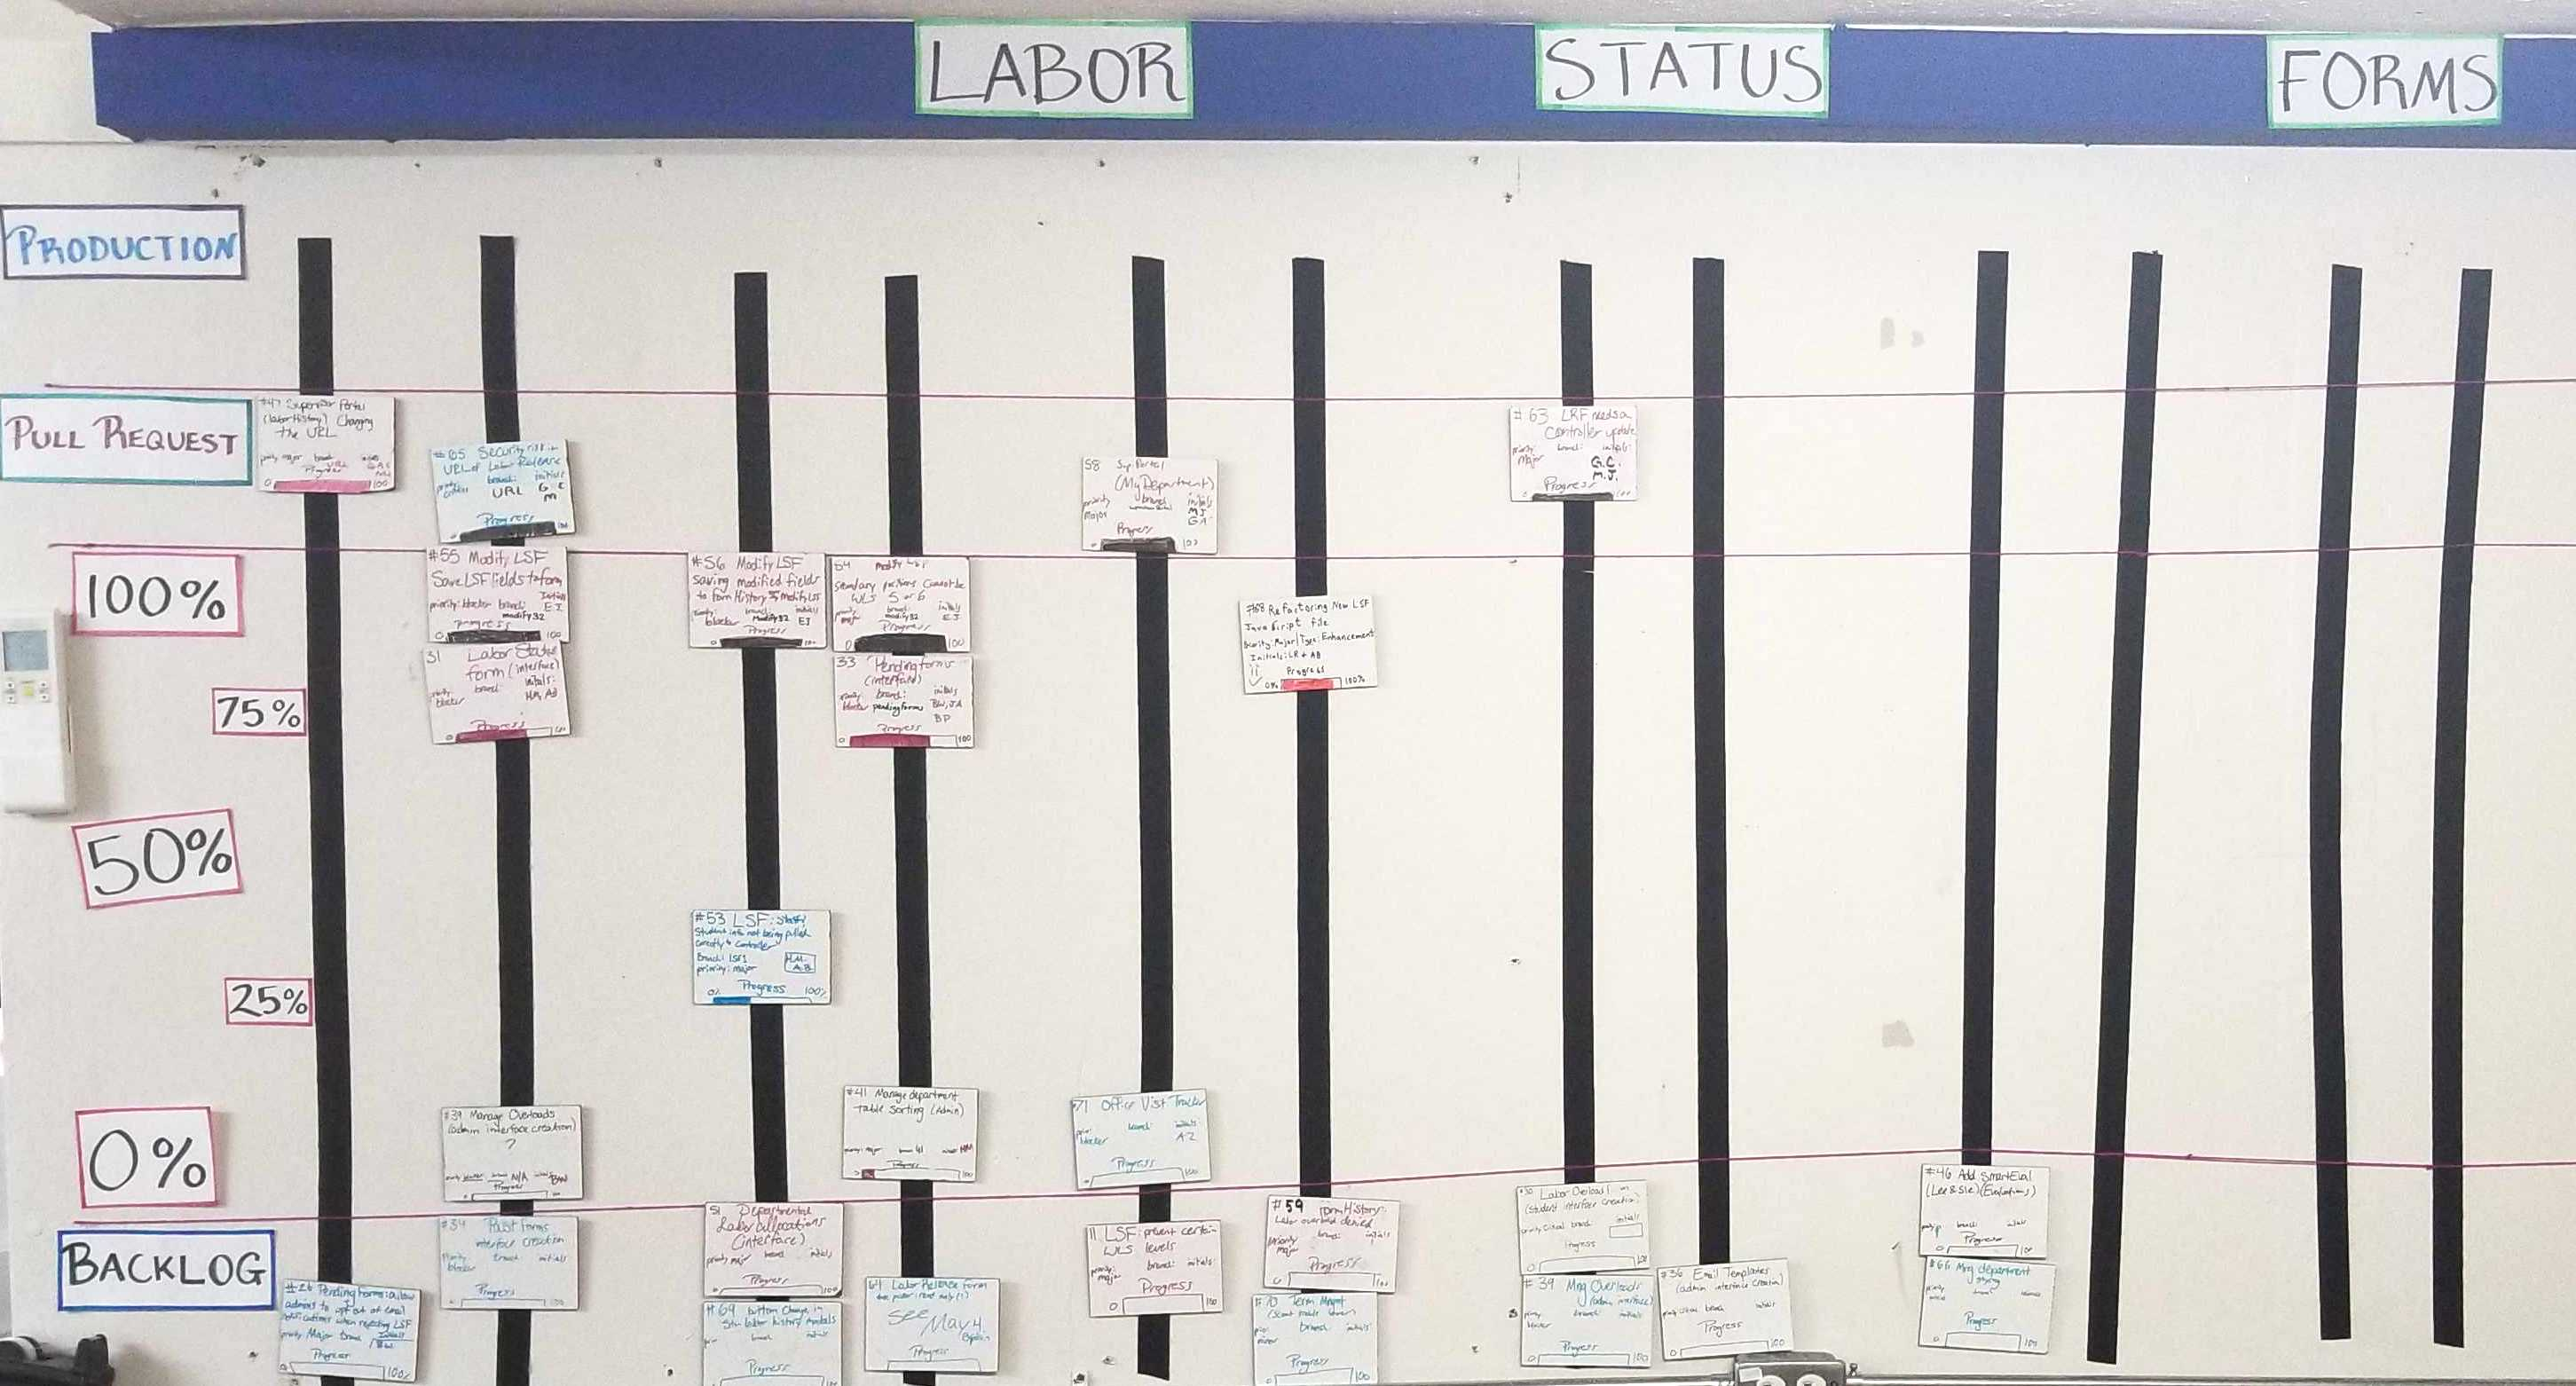
\includegraphics[width=\linewidth]{kanban.jpg}
  \caption{The Student Software Development Framework}
  \Description{The Student Software Development Framework}
\end{figure}

The four Scrum events complemented with Kanban references these events as ``flow-based events'' to acknowledge the importance of managing the teams workflow during these events. The Summer term, when students work for 40 hours a week, is when the team can execute these events to the full extent as the team is able to convene in a way that is comparable to that of a software team that works full-time year round. The Sprint Planning begins when the team decides which customer request will be the central focus for that year. This event is used to outline the work that will be performed during the Sprint. The Development Team uses this time to forecast the range of capabilities that will be developed during the Sprint and to also set the Sprint Goal. The Sprint Goal for the SSDT is to have a beta product available by the end of the Sprint.  When a software is released in beta, the majority of the software requirements have been met, however,there may be small issues that have yet to be addressed.  By releasing beta versions of products, the SSDT and the Product Owner are able to observe most of the functionality of the software that has already and also test for inconsistencies. Close communication with the customers is crucial to the development of the software; staff's needs may change, college policies may update, and staff may move on to jobs elsewhere. As needs change, SSDT can adapt to and account for them.



\paragraph{Sprint Planning \& Paper Prototyping}
Sprint Planning begins with analyzing the current processes that the Product Owner is utilizing*. Asking questions such as, What does the current software that is used to solve their problem look like? How does it work? Are they using any software? Where is the data that needs to be tracked currently being stored? What forms have to be filled out and which people have the authority to approve this process before it is considered to be done and put into action. For instance, if the Product Owner was requesting a software that allows students to add and remove courses to their schedules. The SSDT would need to know how students are currently able to do this task and then make sure to add it to the requirements of the software that is being built. During the SSDT's most recent Sprint, the request that was chosen involved doing an entire refactoring of a live* software.

In order to get a better idea of the functionality of the new software should be implemented, the Development Team begins by going through multiple iterations of paper prototypes. Paper prototyping is a prototyping method in which paper is used to simulate a computer or web application. A paper prototype should hold all of the functionality that the finished user interface of the application will have; from navigation bars, drop down menus, and headers to button clicks and items that will hover on the interface. A person should be able to ``click-through'' the website via the paper prototype. To start this process, screenshots of the old software's interfaces were taken and printed out. Next these interfaces are critiqued* and analyzed to decide which parts are to be kept for the refactoring, which parts will need to be reworked, and which parts will need to be discarded altogether. The purpose of this part of the paper prototyping process is to become familiar with the current software so that the team can adequately build a better software. The team looks for things* such as bugs, broken links, slow page loading, poor user design, etc. and makes a note of these issue to ensure that they are addressed in the new software. After the individual interfaces of the previous software have been discussed and analyzed, the team divides the different interfaces into two categories: Main and Administrative. Main interfaces are the web pages that all users of the application will be able to see whilst Administrative web pages will only be accessed by system administrators, such as BC staff and SSDT's supervisor.

Next the team breaks down the interfaces into issues in which the team will tackle* in pairs. The pair of developers then begins to design the interface that they had chosen from the interfaces that needed to be refactored. Each time a pair from the team believes that they have successfully created a valid* paper prototype, it is then tested for usability. Paper prototyping testing occurs* in  the same way that a fully functional software would be tested, the person testing the paper interface will treat it as such. The tester will ``click'' on different components of the interface and the designers will physically move parts and replace parts of the paper interface in order to replicate how the real software would respond. The pair who designed the interface will take notes as the tester navigates their paper web page and when the test is complete, they use these notes to redesign and the process is repeated. Paper prototyping is done because ``bug'' and inefficiencies are easier to fix when no coding has been done yet and one can go through many iterations without having to actually having to troubleshoot actual code. The SSDT repeats this process of designing, testing, and re-designing until the entire team is satisfied with the final iteration. After all interfaces have been drafted and prototyped, the process of building the application begins and the team commences the Sprint.

\paragraph{ Daily Scrum \& Sprint}
The SSDT uses the Flask framework to build most of its software, following the MVC architectural model. Flask is a web framework that uses Python and Jinja; it is designed to make the start up of web applications faster and easier. It also allows developers to decide what tools and libraries they would like to use for their web application. MVC is architectural model that separates an application into three main logical components: the Model, the View, and the Controller. The Model represent the data and the logic that the user works with in the application. The View is the is composed of all of the User Interface (UI) parts of the application meaning the parts of the application that you can physically see. The Controller is the bridge between the Model and the View; it processes all of the logic, handles requests, manipulates data, and renders the output of the View. All but two applications built by the SSDT were implemented using Flask MVC features. The Sprint is set for 6 weeks with the goal of completing many of the main interfaces in order to have a demo available for  the Product Owner to preview and test.

During the Sprint, the team convenes everyday in the morning in order to touch base with each of the pairs within the team and get an idea of their progress. During the Scrum meeting, the smaller teams tell what the have accomplished since the last meeting, what they will begin to work on next and what they will be completing before the next Scrum meeting, and where they are stuck or if any obstacles got in the way of completing their previous work. Scrum meeting (also called the Daily Stand-Up) is for quick communication purposes and should take no longer than 15 minutes. Sometimes small demos are done during the Scrum meeting in order to get the entire teams' input on certain features before proceeding. The programmers are expected to do a ``DDS'' in a team collaboration application called Slack, DDS stands for Did, Doing, and Stuck. During the Academic Year, these updates serve to compensate the lack of daily Scrum meetings; all students are not available at the same time while classes are in session. Team leaders examine the DDS reports to ensure progress is steady as well as evaluate who needs guidance. These updates also aid in communication between team members if they happen to not see each other. Instead of having a daily Scrum, we instead have a weekly Labor Meeting in which we present and evaluate the team's progress and state in production.

\paragraph{SPRINT REVIEW}
The Sprint Review's purpose is to inspect the amount of work that was completed during the Sprint and measure the amount of work needs to be completed for the next Sprint. The SSDT uses a version control application called GitHub that allows them to edit parts of the software using a copy of the application  in their own environment without interfering with the main program. When the Sprint is completed, the parts of the application that were successfully finalized during the Sprint are merged into the main program. This will allow the team to then create another copy of the main program that now has the new changes and fixes to include in the next Sprint. After the Sprint is completed, the team does an overall demonstration to present the work that they have completed during the Sprint.  After the team demonstration, the Product Owner is brought in so that the team can present the work that has been completed so far. It is important that the Product Owner also participates in the Review; their job is to make sure the work so far meets their criteria and requirements. They also have the authority to reject part of the application, suggest modifications to what has been built, or request a feature be added to the application. The feedback from the Product Owner during this stage is essential as it defines new criteria for the next wave of implementation.

The Review is also used to help set goals for the next iteration. The team holds another meeting to discuss what issues and features were supposed to be completed by the end of the Sprint, but did not. Of those issues, how close are they to being completed and what is a realistic goal that be set for completion in the next Sprint. The SSDT will also review the work that was added during the Sprint or the work was removed. This will give the team insights about what goals may have been too ambitious for the Sprint deadline and what goals could have had more tasks added to them. The Review helps the SSDT to transparently assess the capabilities of the team.

\paragraph{SPRINT RETROSPECTIVE}
This is the final meeting after the Sprint in which the team discusses the overall process and performance of the Sprint. The Sprint Retrospective provides an opportunity for the SSDT and the Scrum Master to strategize ways to improve their methods and approaches for the next Sprint. The objective of this part of the Scrum process is not to focus so much on the work itself but to evaluate the processes of the team. During the meeting, the team finds what activities worked well and should continue to be used in the future, what went wrong during the Sprint, and what could be improved for the next iteration. This meeting is not, however, designed to assess the performance of an individual or to penalize anyone for any shortcomings. The intention of the Retrospective is to gather information about ways to improve the next Sprint. During this discussion, the team openly explores the difficulties and challenges faced during implementation. The team's strengths and triumphs are examined alongside the setbacks to better prepare for these challenges in the future.

\subsubsection{The Academic Term} 
The Fall and Spring terms are both comprised 16 weeks* where most students work at least 10 hours a week. Upperclassmen students can work up to 15 hours a week, if permissible. In addition to class scheduling occupying the students' weekly routines, the weekly labor restrictions follow the guidelines established by the labor program at the institution.


"MOVE ME" ``The SDDT at our institution was established over four years ago with the Student Software Development Initiative by a Computer Science faculty member.''

"DONT THINK WE NEED THIS" ``Students learn real-world work skills such as time management, and responsibility. Some students move up into positions of leadership and build those skills. Between classes, extracurriculars, and secondary labor positions, SSDT's staff dedicate time to their labor hours.''